\documentclass[12pt,openany]{report}
\def\tit{DNA Sequence}
\date{\today}
\makeatletter
\let\datename\@date
\makeatother
\def\authorname{Simone Lidonnici - (2061343)\\Marco Casu - (2041262)}



%Include------------------------------------------------
\usepackage[italian]{babel}
\usepackage{array}
\usepackage{booktabs}
\usepackage{colortbl}
\usepackage[paper=a4paper,left=20mm,right=20mm,bottom=25mm,top=25mm]{geometry}
\usepackage{graphicx}
\usepackage{bookmark}
\usepackage[listings,breakable]{tcolorbox}
\tcbuselibrary{skins}
\usepackage{fancyhdr}
\usepackage[absolute,overlay]{textpos}
%-------------------------------------------------------




%Stile pagina
\raggedbottom
\pagestyle{fancy}
\setlength{\headheight}{15pt}
\fancyhead[L]{\nouppercase{\leftmark}}
\fancyhead[R]{\ifnum\value{chapter}>0{\nouppercase{\rightmark}}\fi}
\fancyfoot[C]{\thepage}
%------------------------------------------------


\renewcommand{\thesection}{\arabic{section}}
\definecolor{Sapienza}{RGB}{131,31,48}


\begin{document}
%INIZIO PRIMA PAGINA
\begin{titlepage}
    \begin{center}
        
\includegraphics[width=0.5\textwidth]{images/Sapienza_logo.png}
    \end{center}
    \centering\Large \textbf{\color{Sapienza}{Facoltà di Ingegneria dell'Informazione, Informatica e Statistica\\Dipartimento di Informatica}}
    \vspace{4cm}
    \begin{tcolorbox}[enhanced, width=\textwidth, colframe=Sapienza, colback=white, halign=flush center, sharp corners=all, boxrule=1mm, bottom=5mm, top=5mm]
        \Huge\textbf{\tit}
    \end{tcolorbox}
    \begin{textblock*}{\textwidth}[0.5,0](0.5\pdfpagewidth,20cm)
        \centering\large\textbf{Autori:}\\\authorname
    \end{textblock*}
    \vfill
    \centering\large\datename
\end{titlepage}
%FINE PRIMA PAGINA

\section{Introduzione}
Le parti principali di codice da parallelizzare sono la creazione della sequenza e la ricerca dei pattern. Per sequenze medio-piccole quest'ultima compone la maggior parte del tempo di compilazione, mentre aumentando la grandezza della sequenza (nell'ordine dei miliardi), la maggior parte del tempo è richiesto per generare la sequenza. Da notare che nel programma sequenziale il tempo non conta la generazione di quest'ultima mentre nei programmi paralleli (MPI, OpenMP, CUDA e MPI+OpenMP) si, cosa che causa una diminuzione dello speedup.
\subsection{Test e calcolo dello speedup}
Le varie versioni del programma sono state testate sul cluster eseguendo 10 test e controllando il tempo medio di essi, scartando dal calcolo della media il caso peggiore ed il caso migliore, in particolare il test è stato eseguito con i seguenti parametri:
\begin{center}
    \texttt{500000 0.35 0.2 0.25 30000 2000 1000 30000 2000 1000 500 100 M 4353435}
\end{center}

\newpage
\section{MPI}
Nel programma MPI la ricerca dei pattern è stata distribuita uniformemente tra i rank, se $t$ è il numero dei processi, allora ognuno ricercherà $\lceil \frac{n}{t}\rceil$ pattern, con $n$ numero totale di pattern (sia sample che random). Se $\frac{n}{t}$ non è un numero intero, l'ultimo rank ricercherà meno pattern rispetto ad ogni altro. Per avere poi il valore corretto dei pattern trovati e dei pattern in ogni punto della sequenza vengono eseguite delle collettive \texttt{MPI\_Reduce} su \texttt{seq\_matches} e \texttt{pat\_found}.

\bigskip 
Riguardo la generazione della sequenza,
è stato osservato che, questa, risulta  più veloce nella versione sequenziale, anche se viene adoperato un singolo thread, la funzione\\ \texttt{generate\_random\_sequence} impiega sempre meno tempo ad essere eseguita nella versione sequenziale piuttosto che in quella parallela. Sono stati tentati due approcci:
\begin{itemize}
    \item Si è inizialmente provato a far generare l'intera sequenza ad un solo processo, per poi eseguire una \texttt{MPI\_Broadcast}, condividendola a tutti gli altri processi. Tale versione si è rivelata più veloce della versione iniziale (in cui ogni rank genera autonomamente la sequenza) ma comunque più lenta della versione sequenziale.
    \item La seconda opzione, presente nel file finale, è stata quella di dividere la sequenza tra i vari rank, nello stesso modo in cui vengono divisi i pattern e poi eseguire una \texttt{MPI\_Allreduce} per far avere a tutti i rank la sequenza completa. Data la natura puramente sequenziale delle funzioni rng, ogni rank esegue un \texttt{rng\_skip} per poter iniziare a generare i suoi numeri random da un punto avanzato della sequenza.
\end{itemize}
Di seguito si può vedere il grafico dei tempi e dello speed up in relazione al numero di processi MPI, i test sono stati eseguiti con il numero massimo di processi su un nodo (32) e aumentando i nodi progressivamente:
\begin{center}
    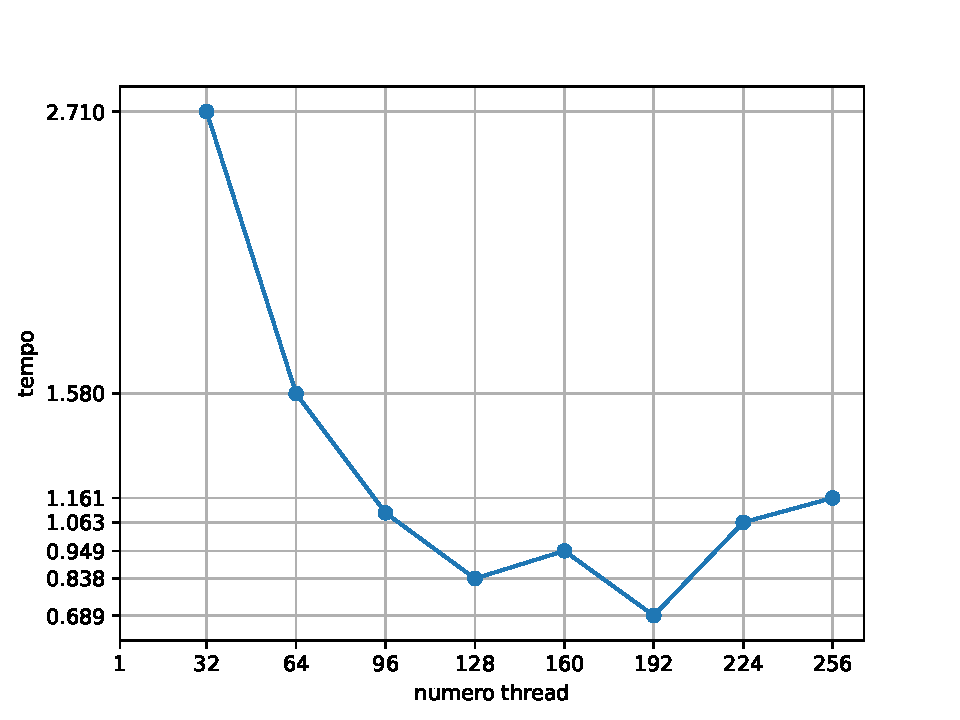
\includegraphics[width=0.48\textwidth ]{images/tempi_MPI.pdf}
    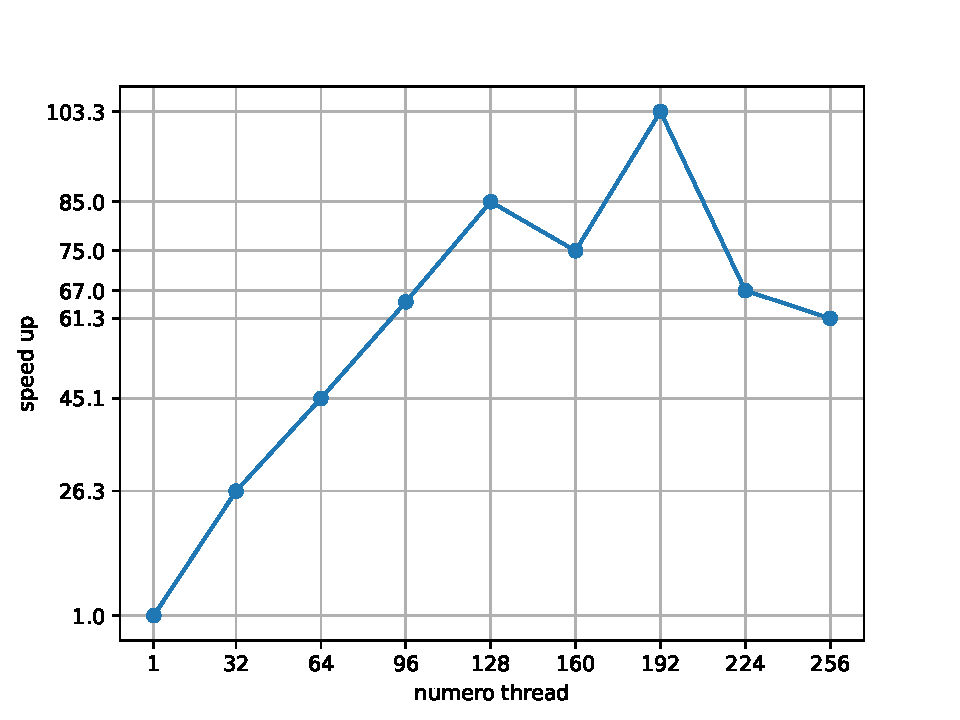
\includegraphics[width=0.48\textwidth ]{images/speedup_MPI.pdf}
\end{center}
L'esecuzione sequenziale (non riportata nel grafico) ha impiegato 71.27 secondi.
\newpage
Se si vogliono consultare le informazioni in maniera più pratica, si può controllare la seguente tabella:
\begin{center}
    \begin{tabular}{|c|c|c|c|}
        \hline
        \rowcolor[HTML]{EFEFEF} 
        numero di processi & tempo   & speedup & efficienza   \\ \hline
        sequenziale      & 71.27 & 1         & 1 \\ \hline
        32               & 2.71  & 26.27 & 0.82 \\ \hline
        64               & 1.57   & 45.07 & 0.70 \\ \hline
        96               & 1.10  & 64.64 & 0.67 \\ \hline
        128              & 0.83  & 84.97 & 0.66 \\ \hline
        160              & 0.94  & 75.03 & 0.46 \\ \hline
        192              & 0.68    & 103.28 & 0.53 \\ \hline
        224              & 1.06  & 66.95 & 0.29 \\ \hline
        256              & 1.16  & 61.32  & 0.23 \\ \hline
    \end{tabular}
\end{center}
\textbf{Nota} : il tempo medio per l'esecuzione con 256 rank risulta maggiore al tempo medio con 96 rank, anche se il caso migliore risulta più rapido, non è chiaro se l'aleatoreità delle differenze di tempo fra differenti esecuzioni del programma sia dovuta al sovraccarico del cluster, sono riportati qui sotto i grafici e la tabella dei tempi di esecuzione nei \textit{casi migliori}:
\begin{center}
    \begin{tabular}{|c|c|c|c|}
        \hline
        \rowcolor[HTML]{EFEFEF} 
        numero di processi & tempo& speedup & efficienza  \\ \hline
        sequenziale      & 71.27 & 1 & 1\\ \hline
        32               & 2.29  & 31.01 & 0.96\\ \hline
        64               & 1.19  & 59.71 & 0.93\\ \hline
        96               & 0.82  & 86.91 & 0.90\\ \hline
        128              & 0.78  & 91.37 & 0.71\\ \hline
        160              & 0.63  & 113.13 & 0.70\\ \hline
        192              & 0.52  & 137.06 & 0.71\\ \hline
        224              & 0.50  & 142.54 & 0.63\\ \hline
        256              & 0.44  & 161.98 & 0.63\\ \hline
    \end{tabular}\\ 
    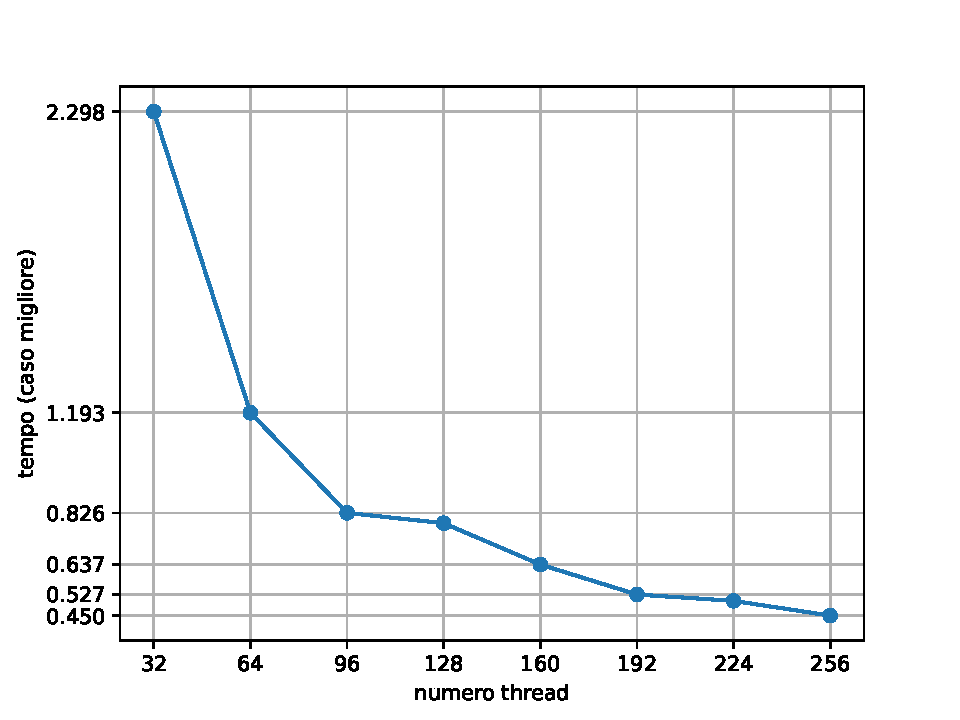
\includegraphics[width=0.6\textwidth ]{images/tempi_MPI_bestcase.pdf}
\end{center}
Si noti come nel caso migliore, all'aumentare dei thread il tempo va sempre diminuendo.



\newpage
\section{OpenMP}
Nel programma OpenMP per quanto riguarda la ricerca dei pattern abbiamo creato delle variabili \texttt{pat\_matches} e \texttt{seq\_matches} private per ogni thread e abbiamo parallelizzato solamente il ciclo più esterno, tramite un \texttt{\#pragma omp for}, questo perché i tre cicli non potevano essere collassati in uno unico data la presenza di \texttt{break} al loro interno.
\bigskip

Dopo il ciclo \texttt{for} relativo alla ricerca dei pattern ogni thread avrà operato sulle proprie copie private di \texttt{pat\_matches} e \texttt{seq\_matches}. Sarà necessario collossare i risultati parziali ottenuti da ogni thread, sommandone i valori.
A tal proposito, sarà necessario sequenziare una porzione di codice con la direttiva \texttt{\#pragma omp critical}, in cui ogni thread sommerà i valori di \texttt{pat\_matches} e \texttt{seq\_matches} per avere i valori finali corretti.\bigskip

Per quanto riguarda invece la creazione della sequenza abbiamo usato lo stesso approccio di MPI, cioè dividerla in parti uguali in base all'id del thread e far eseguire ad ogni thread \texttt{rng\_skip} fino al punto dove deve iniziare a generare i propri numeri random. Per impostare il numero di thread è stato aggiunto un argomento in input, in modo da poterli impostare da linea di comando.\bigskip


Di seguito si può vedere il grafico dei tempi e dello speedup in relazione al numero di thread, i test sono stati eseguiti aumentando il numero di thread progressivamente:
\begin{center}
    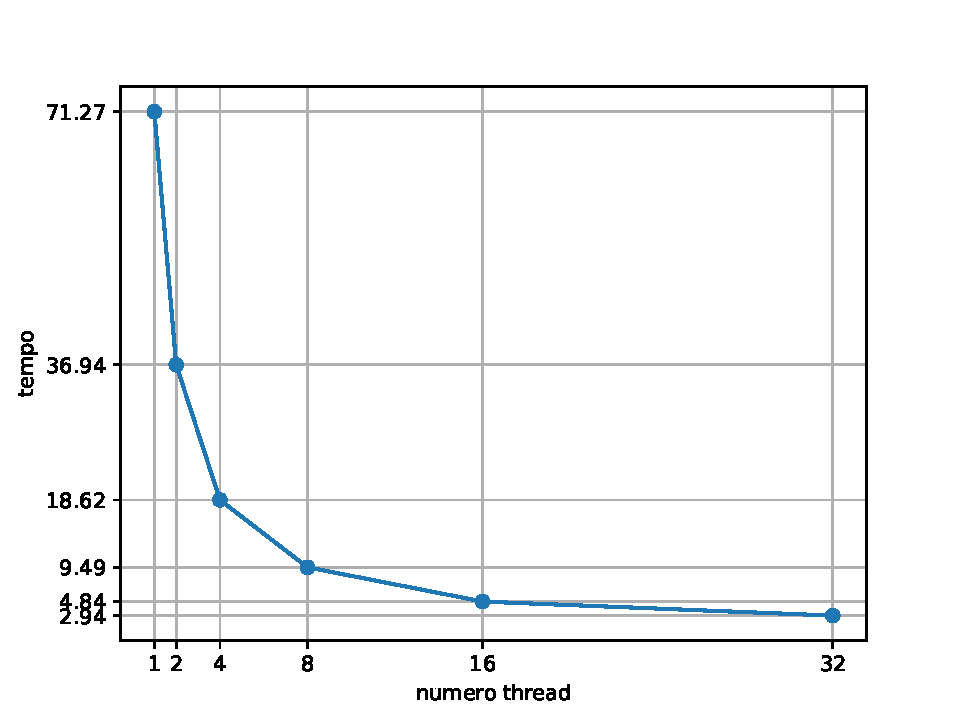
\includegraphics[width=0.5\textwidth ]{images/tempi_OpenMP.pdf}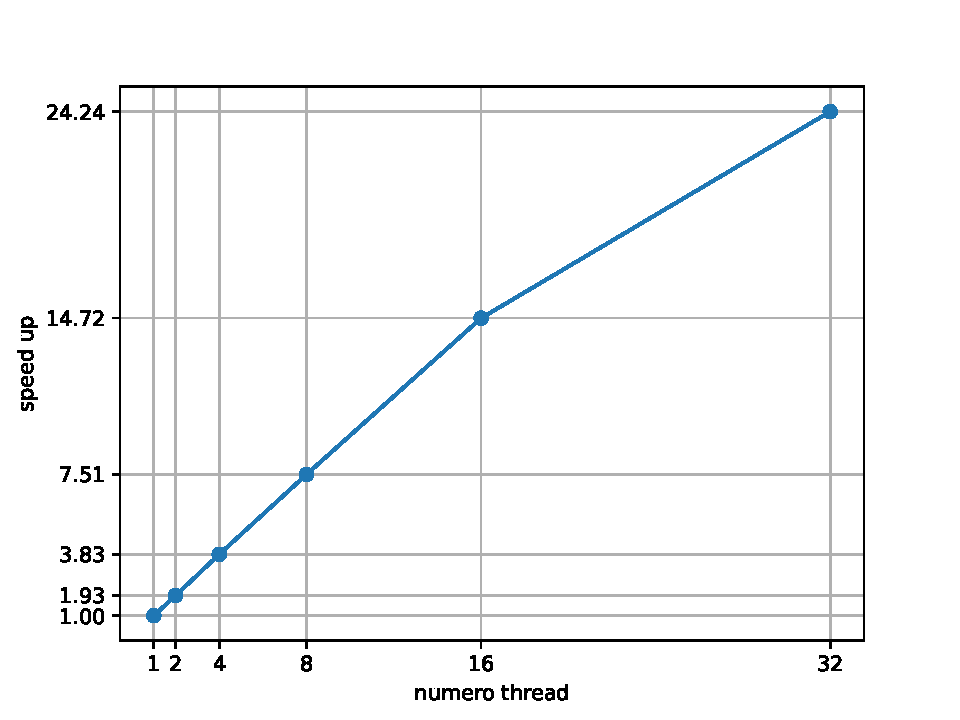
\includegraphics[width=0.5\textwidth ]{images/speedup_OpenMP.pdf}
\end{center}
Si osservi come la decrescita del tempo impiegato a terminare il programma è inizialmente esponenziale. In seguito, è riportata la tabella dei tempi e dello speed up:
\begin{center}
    \begin{tabular}{|c|c|c|c|}
        \hline
        \rowcolor[HTML]{EFEFEF} 
        numero di  thread & tempo & speedup & efficienza\\ \hline
        sequenziale       & 71.27 & 1       & 1 \\ \hline
        2                 & 36.94 & 1.92    & 0.96 \\ \hline
        4                 & 18.62 & 3.82    & 0.95 \\ \hline
        8                 & 9.48  & 7.51    & 0.93 \\ \hline
        16                & 4.84  & 14.71   & 0.91 \\ \hline
        32                & 2.93  & 24.24   & 0.75 \\ \hline
        \end{tabular}
\end{center}
Si noti come a parità di processi (nel caso con 32 thread), l'esecuzione parallela in MPI risulta più efficiente rispetto quella in OpenMP.


\end{document}